\chapter{Arhitektura i dizajn sustava}
		Arhitektura naše aplikacije, može se podijeliti na sljedeće komponente
	\begin{itemize}
		\item 	Server strana (\textit{backend})
		\item 	Klijent strana (\textit{frontend})
		\item 	Baza podataka (\textit{db})		
	\end{itemize}
	\textbf{Serverska strana} glavna je komponenta naše aplikacije. U njoj se nalazi programska logika koja se brine da se korisniku isporuči ono što je zatražio i da aplikacija radi u skladu sa zahtjevima. Komunikacija prema klijentskoj strani ostvarena je korištenjem GraphQL-a (za manipulaciju s API-jem), a komunikacija prema bazi podataka ORM-om (Object-Relational Mapping). Također smo koristili razred Prisma kojem se predaju parametri SQL upita. Prisma je biblioteka sa serverske strane koja pomaže pri čitanju i pisanju podataka u i iz baze podataka na siguran način (štiti od SQL injekcija).
	
	\textbf{Baza podataka} koju smo koristili je PostgreSQL. Kako bi izbjegli programske greške u SQLu te potencijalne ranjivosti (npr. SQL injekcija), za komunikaciju s bazom koristili smo \textit{TypeORM} kako bi programer izbjegao greške u SQL jeziku. \textit{TypeOrm} je podvrsta radnog okvira ORM prilagođen TypeScriptu i JavaScriptu. Kroz \textit{TypeORM} dobili smo i sustav za verzioniranje baze podataka "migracije" tako da možemo lakše i sigurnije raditi izmjene na bazi te dijeliti te izmjene između programera u timu i produkcijskih servera. 
	
	\textbf{Klijentska strana} je pruža grafičko sučelje za olakšan i intuitivan pristup uslugama aplikacije. Ovu komponentu možemo zamisliti kao posrednika u komunikaciji između korisnika i serverske strane aplikacije. U našem slučaju klijentska strana implementirana je kao SPA (Single Page Application) s \textit{React}-om. \textit{React} je JavaScript knjižnica koja olakšava oblikovanje korisničkog sučelja.\\
	
	\begin{figure}[H]
		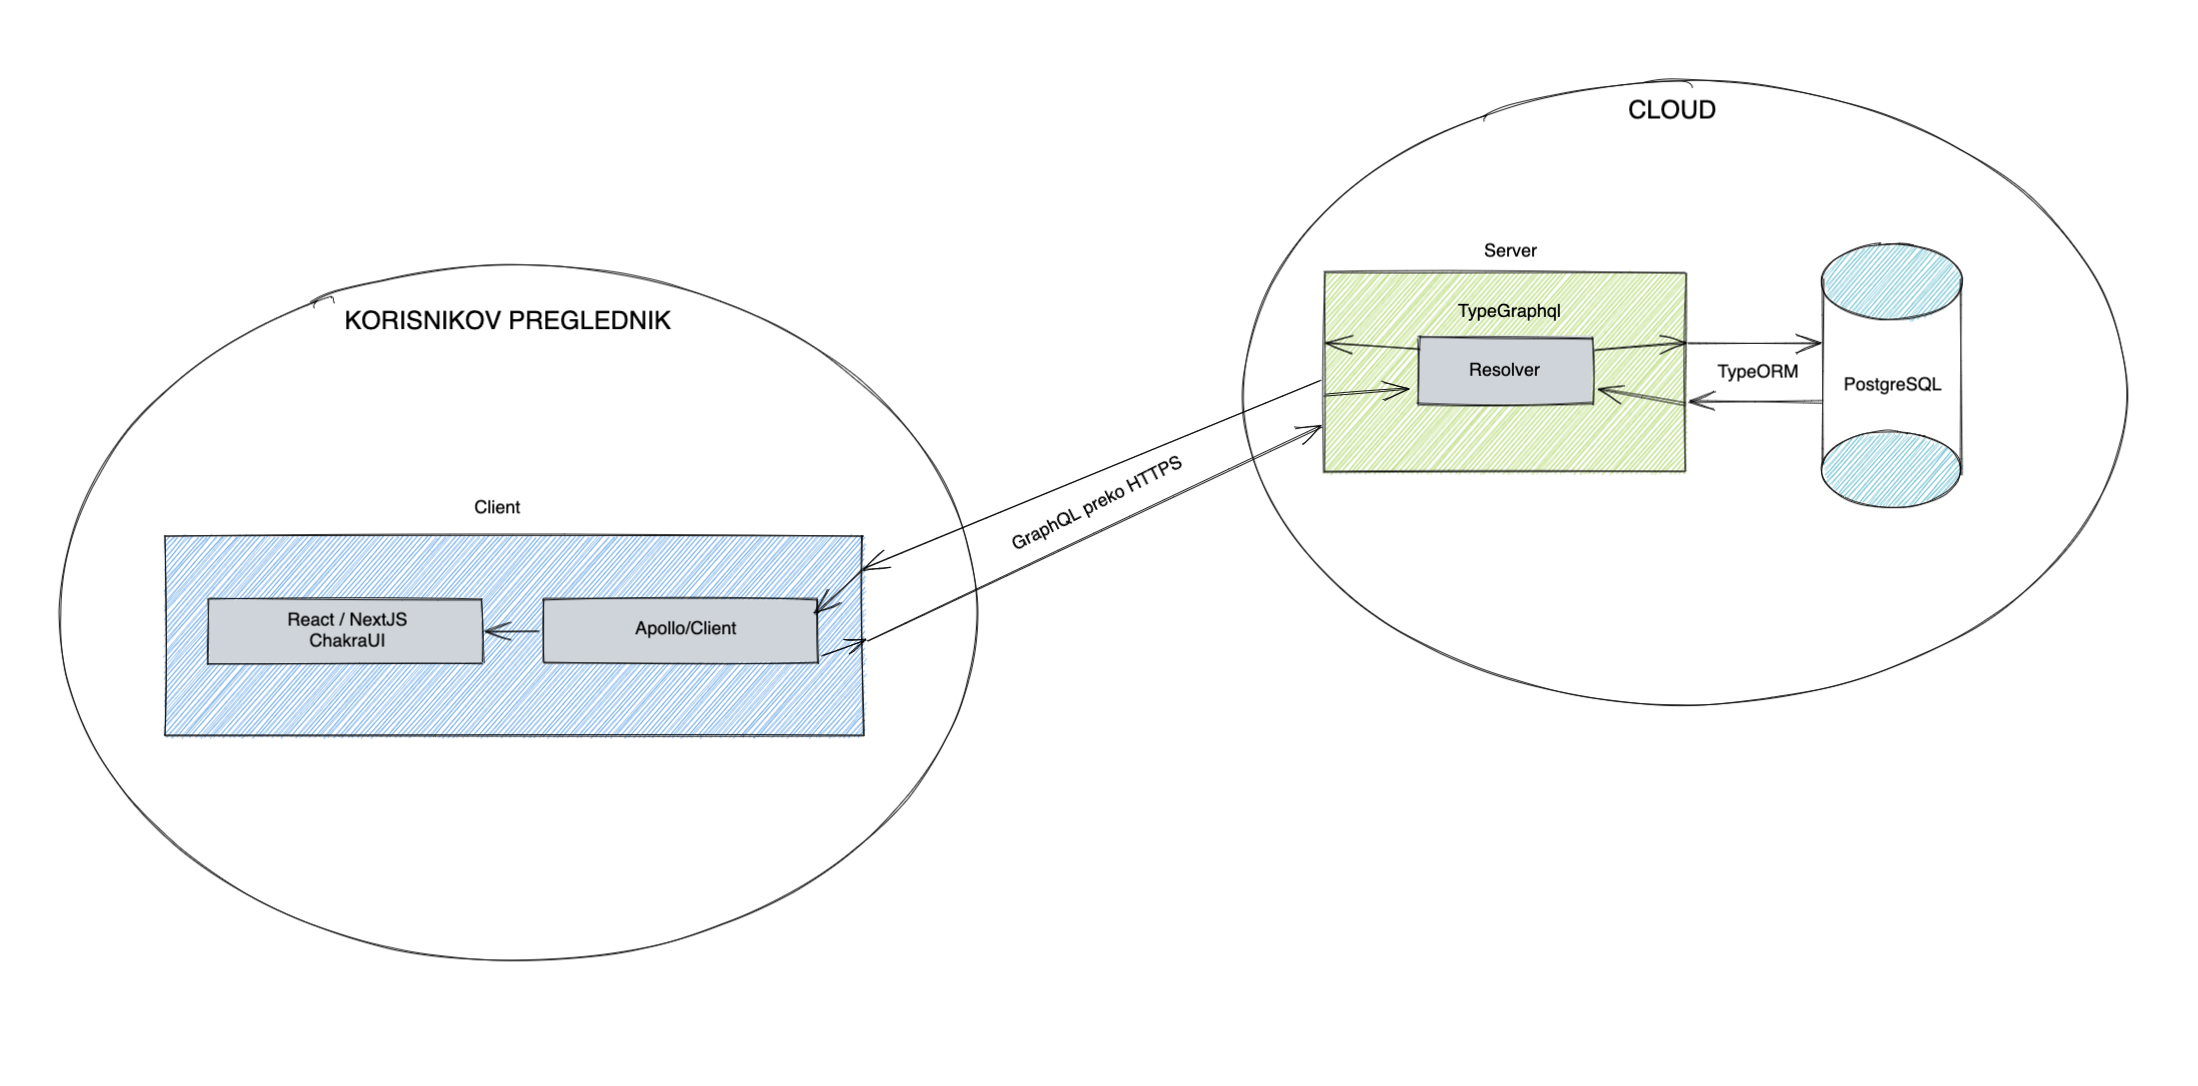
\includegraphics[width=\textwidth]{slike/arhitekturaDijagram.png} 
		\caption{Model arhitekture}
		\label{fig:arhitektura} 
	\end{figure}

				
		\section{Baza podataka}
		
		U našem sustavu korisimo PostgreSQL relacijsku bazu podataka za spremanje informacija o korisnicima (administratori i seizmolozi/znanstvenici), potresima i upitnicima te odgovorima iz tih upitnika. Zadaća baze podataka brza je i jednostavna pohrana, izmjena i dohvat podataka za daljnju obradu. Podaci će biti pohranjeni u tablice koje imaju svoje ime i atribute te će svaki entitet imati svoj primarni ključ, jedinstvenu
		oznaku svake n-torke koja ne smije imati vrijednost ”null”.
		U bazi podataka imamo sljedeće entitete:
		\begin{itemize}
			\item 	users
			\item 	earthquakes
			\item 	surveys
			\item   survey\_responses
		\end{itemize}

			\subsection{Opis tablica}
			
				Tablica u kojoj se spremaju pristupni podaci te uloge korisnika u sustavu. Spremamo vrijeme kreiranja i izmjene podataka o korisniku.
				Svaki korisnik ima svoju e-mail adresu te hash svoje lozinke te ulogu - korisnik može biti ili administrator ili seizmolog/znanstvenik.
				U ovoj tablici također spremamo informaciju je li korisnik promijenio inicijalnu lozinku.
				\begin{longtblr}[
					label=none,
					entry=none
					]{
						width = \textwidth,
						colspec={|X[7,l]|X[7, l]|X[20, l]|}, 
						rowhead = 1,
					} %definicija širine tablice, širine stupaca, poravnanje i broja redaka naslova tablice
					\hline \multicolumn{3}{|c|}{\textbf{users}}	 \\ \hline[3pt]
					\SetCell{LightGreen}id & INT	&  	id korisnika  	\\ \hline
					created\_at	& TIMESTAMP &  vremenski žig kada je korisnik stvoren	\\ \hline 
					updated\_at	& TIMESTAMP &  vremenski žig kada je korisnik izmijenjen 	\\ \hline 
					email & VARCHAR &  email adresa korisnika \\ \hline 
					password\_hash & VARCHAR &  lozinka korisnika spremljena kao hash \\ \hline 
					role & Enum:UserRole &  uloga korisnika (admin i seizmolog) \\ \hline 
					changedPassword & BOOLEAN & je li korisnik promijenio inicijalnu lozinku
				\end{longtblr}

				Tablica u kojoj se spremaju prošli potresi, svaki potres može imati 0:n upitnika koje su građani ispunili. Spremamo vrijeme kreiranja i izmjene potresa. 
				Podaci koje spremamo o potresu su naziv potresa, intenzitet, lokacija kao geografska širina i dužina te vrijeme kada se potres dogodio i kada je potres bio arhiviran.
				\begin{longtblr}[
					label=none,
					entry=none
					]{
						width = \textwidth,
						colspec={|X[7,l]|X[7, l]|X[20, l]|}, 
						rowhead = 1,
					} %definicija širine tablice, širine stupaca, poravnanje i broja redaka naslova tablice
					\hline \multicolumn{3}{|c|}{\textbf{earthquakes}}	 \\ \hline[3pt]
					\SetCell{LightGreen}id & INT	&  	id potresa  	\\ \hline
					created\_at	& TIMESTAMP &  vremenski žig kada je potres stvoren	\\ \hline 
					updated\_at	& TIMESTAMP &  vremenski žig kada je potres izmijenjen 	\\ \hline 
					name & VARCHAR &  naziv potresa \\ \hline 
					strength & REAL &  jačina potresa \\ \hline 
					epicenter\_lat & REAL &  geografska širina epicentra \\ \hline 
					epicenter\_lng & REAL &  geografska dužina epicentra \\ \hline 
					date	& TIMESTAMP &  vremenski žig kada se potres dogodio 	\\ \hline 
					archived\_at	& TIMESTAMP &  vremenski žig kada je potres arhiviran 	\\ \hline 
				\end{longtblr}

				Tablica u kojoj se nalaze ispunjeni upitnici. Spremamo vrijeme kreiranja i izmjene upitnika. 
				U bazi lokaciju korisnika spremamo kao geografsku širinu i dužinu odnosno dva broja, lat i long.
				Također spremamo jačinu potresa koju je osoba osjetila te grad u kojem je upitnik ispunjen.
				\begin{longtblr}[
					label=none,
					entry=none
					]{
						width = \textwidth,
						colspec={|X[7,l]|X[7, l]|X[20, l]|}, 
						rowhead = 1,
					} %definicija širine tablice, širine stupaca, poravnanje i broja redaka naslova tablice
					\hline \multicolumn{3}{|c|}{\textbf{surveys}}	 \\ \hline[3pt]
					\SetCell{LightGreen}id & INT	&  	id upitnika  	\\ \hline
					created\_at	& TIMESTAMP &  vremenski žig kada je upitnik stvoren	\\ \hline 
					updated\_at	& TIMESTAMP &  vremenski žig kada je upitnik izmijenjen 	\\ \hline 
					lat & REAL &  geografska širina upitnika \\ \hline 
					lng & REAL &  geografska dužina upitnika \\ \hline 
					strength & INT & jačina koju je osoba koja je ispunila upitnik osjetila \\ \hline
					city & VARCHAR & grad u kojem je upitnik ispunjen \\ \hline
					\SetCell{LightBlue}earthquakeId	& INT &  id potresa za koji je ovaj upitnik ispunjen 	\\ \hline 
				\end{longtblr}

				Tablica u kojoj se nalaze odgovori pojedinačnog upitnika. Spremamo vrijeme kreiranja i izmjene svakog odgovora. 
				U aplikaciji pitanja i odgovore imamo spremljene u listi tako da u ovoj tablici imamo indekse pitanja i odgovora.
				\begin{longtblr}[
					label=none,
					entry=none
					]{
						width = \textwidth,
						colspec={|X[7,l]|X[7, l]|X[20, l]|}, 
						rowhead = 1,
					} %definicija širine tablice, širine stupaca, poravnanje i broja redaka naslova tablice
					\hline \multicolumn{3}{|c|}{\textbf{survey\_responses}}	 \\ \hline[3pt]
					\SetCell{LightGreen}id & INT & id odgovora \\ \hline
					created\_at	& TIMESTAMP & vremenski žig kada je odgovor stvoren	\\ \hline 
					updated\_at	& TIMESTAMP & vremenski žig kada je odgovor izmijenjen 	\\ \hline 
					questionId & VARCHAR & oznaka pitanja \\ \hline 
					optionId & VARCHAR & oznaka odgovora \\ \hline 
					\SetCell{LightBlue}surveyId	& INT &  id upitnika za kojem pripada ovaj odgovor 	\\ \hline 
				\end{longtblr}

			
			\subsection{Dijagram baze podataka}

				\begin{figure}[H]
					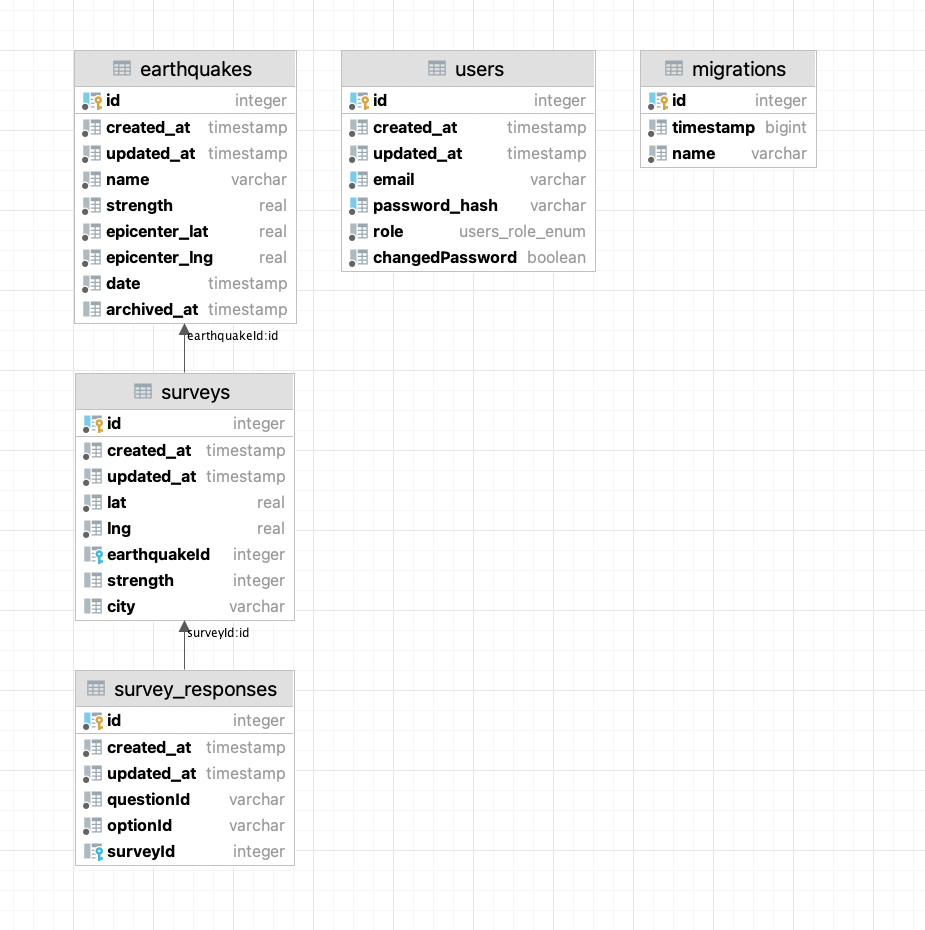
\includegraphics[width=\textwidth]{slike/tectonicDBDiagram.png} 
					\caption{Dijagram baze podataka}
					\label{fig:baza} 
				\end{figure}

			\eject
			
			
		\section{Dijagram razreda}
			
			Svi modeli iz baze podataka izvedeni su iz BaseModel razreda. Taj razred kao atribute ima oznaku (id) te vrijeme kreiranja i zadnje izmjene. 
			Razred BaseModel koristimo zato što svi modeli sadržavaju te iste atribute. 
			Razred User sadrži podatke o korisniku, e-mail, lozinka te je li korisnik administrator ili seizmolog/znanstvenik.
			Razred Earthquake također sadrži atribute za vrijeme kada se potres dogodio, kada je arhivirat, koordinate epicentra, naziv i intenzitet te listu upitnika koje su korisnici ispunili za taj potres.
			Razred Survey opisuje upitnik atributima za ime grada u kojem je upitnik ispunjen (izračunato iz koordinati), potres za koji je upitnik ispunjen, koordinate na kojima je upitnik ispunjen (za računanje epicentra potresa), listu odgovora na pitanja te intenzitet potresa izračunat iz odgovora.
			SurveyResponse predstavlja odgovor na jedno pitanje u upitniku. Sadrži referencu na upitnik kojem pripada te oznake pitanja i odgovora. 
			Popis pitanja i odgovora je spremljen u surveyQuestions datoteci.
			\begin{figure}[H]
				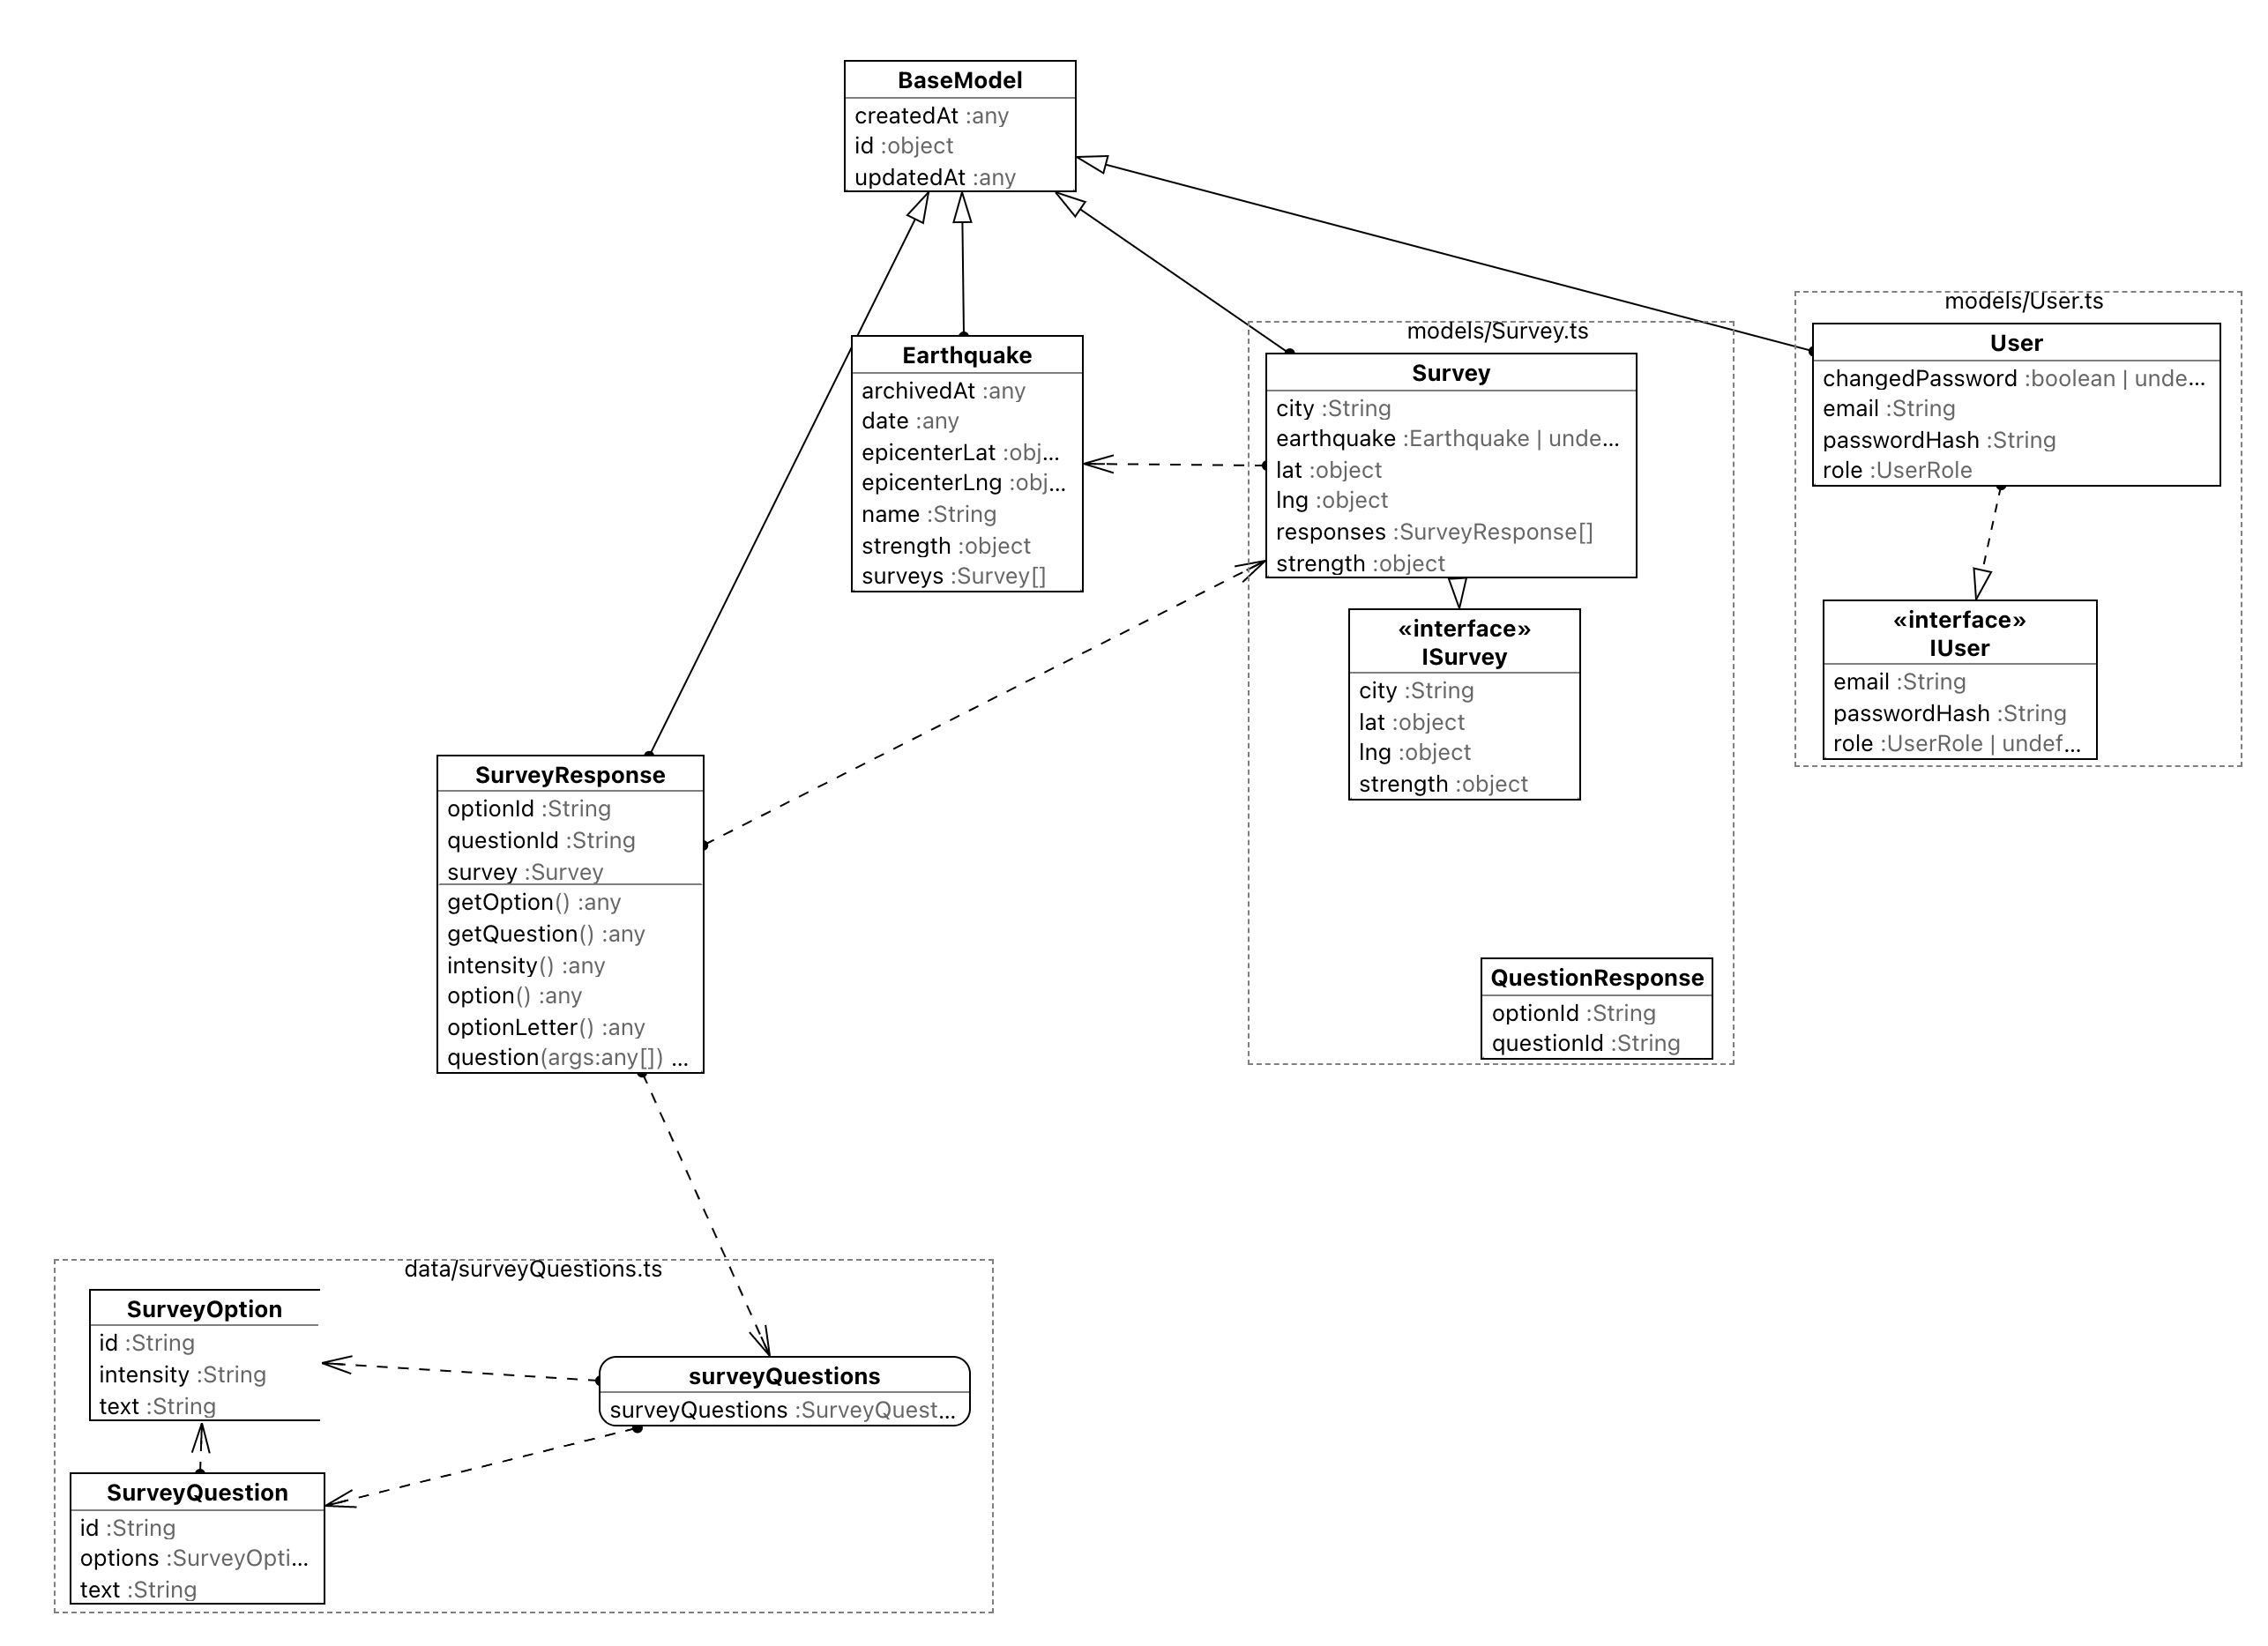
\includegraphics[width=\textwidth]{slike/classdiagram_only_db.png} 
				\caption{Dijagram razreda za modeliranje baze podataka}
				\label{fig:uml_db} 
			\end{figure}

			Dohvaćanje podataka te pisanje novih / modificiranje postojećih smo podijelili po svakom modelu u pojedine graphql resolvere. 
			Za svaki resolver smo posebno napisali razrede koje validiranju inpute te ih koristili u samom resolveru. 
			Svi resolveri osim Cities i SuveryQuestions ovise o bazi te komuniciraju s njom preko svojih modela (Surveys preko Survey modela, itd), 
			dok Cities/SurveyQuestions direktno čitanju pitanja iz fileova. Svi resolveri su importani u resolvers.ts file iz kojeg se jedan array 
			resolvera exporta te dodaje u inicijalizaciju servera koja se odbija u main.ts fileu. U njemu prije pokretanja servera inicijaliziramo 
			konekciju s bazom podataka. Svaki request koji naš HTTP server prihvati prvo prolazi kroz user Middleware gdje se iz headera izvuče JWT 
			token po kojem se dohvati korisnik te se po tome može znati im li korisnik prava pristupati nekim dijelovima aplikacije ili ne.

			\begin{figure}[H]
				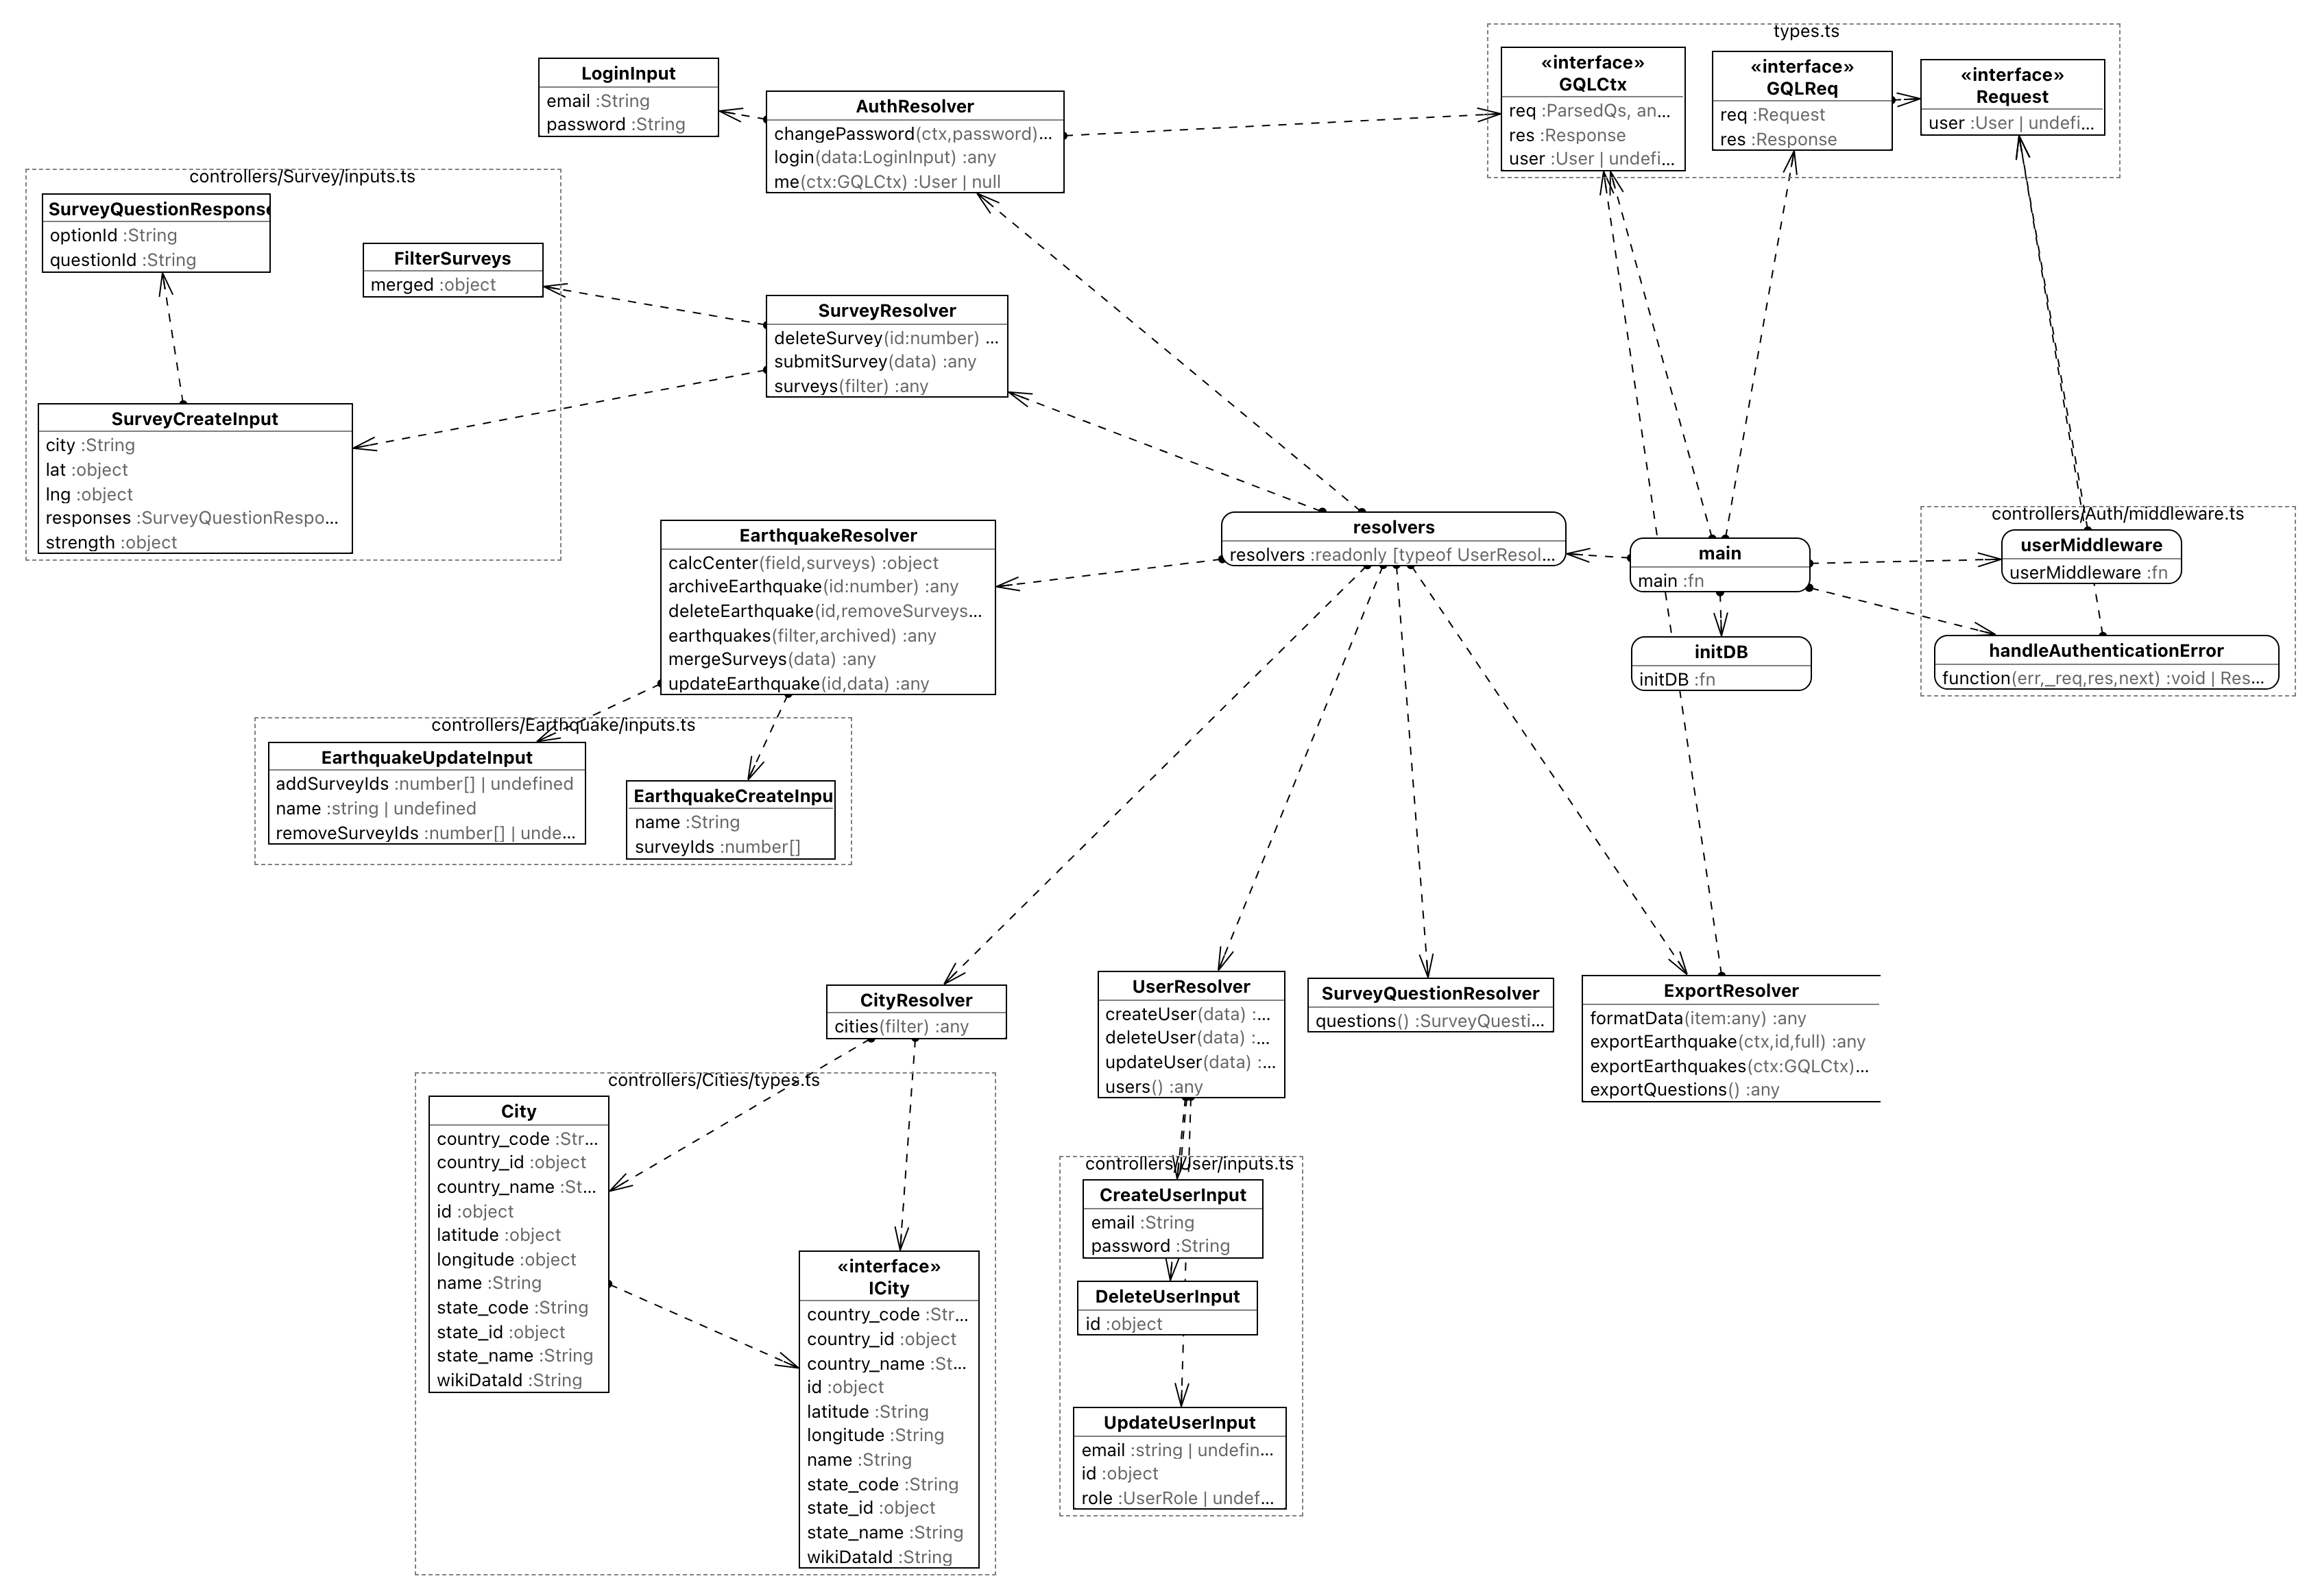
\includegraphics[width=\textwidth]{slike/classdiagram_no_db.png} 
				\caption{Dijagram razreda bez baze podataka}
				\label{fig:uml_no_db} 
			\end{figure}

			\begin{figure}[H]
				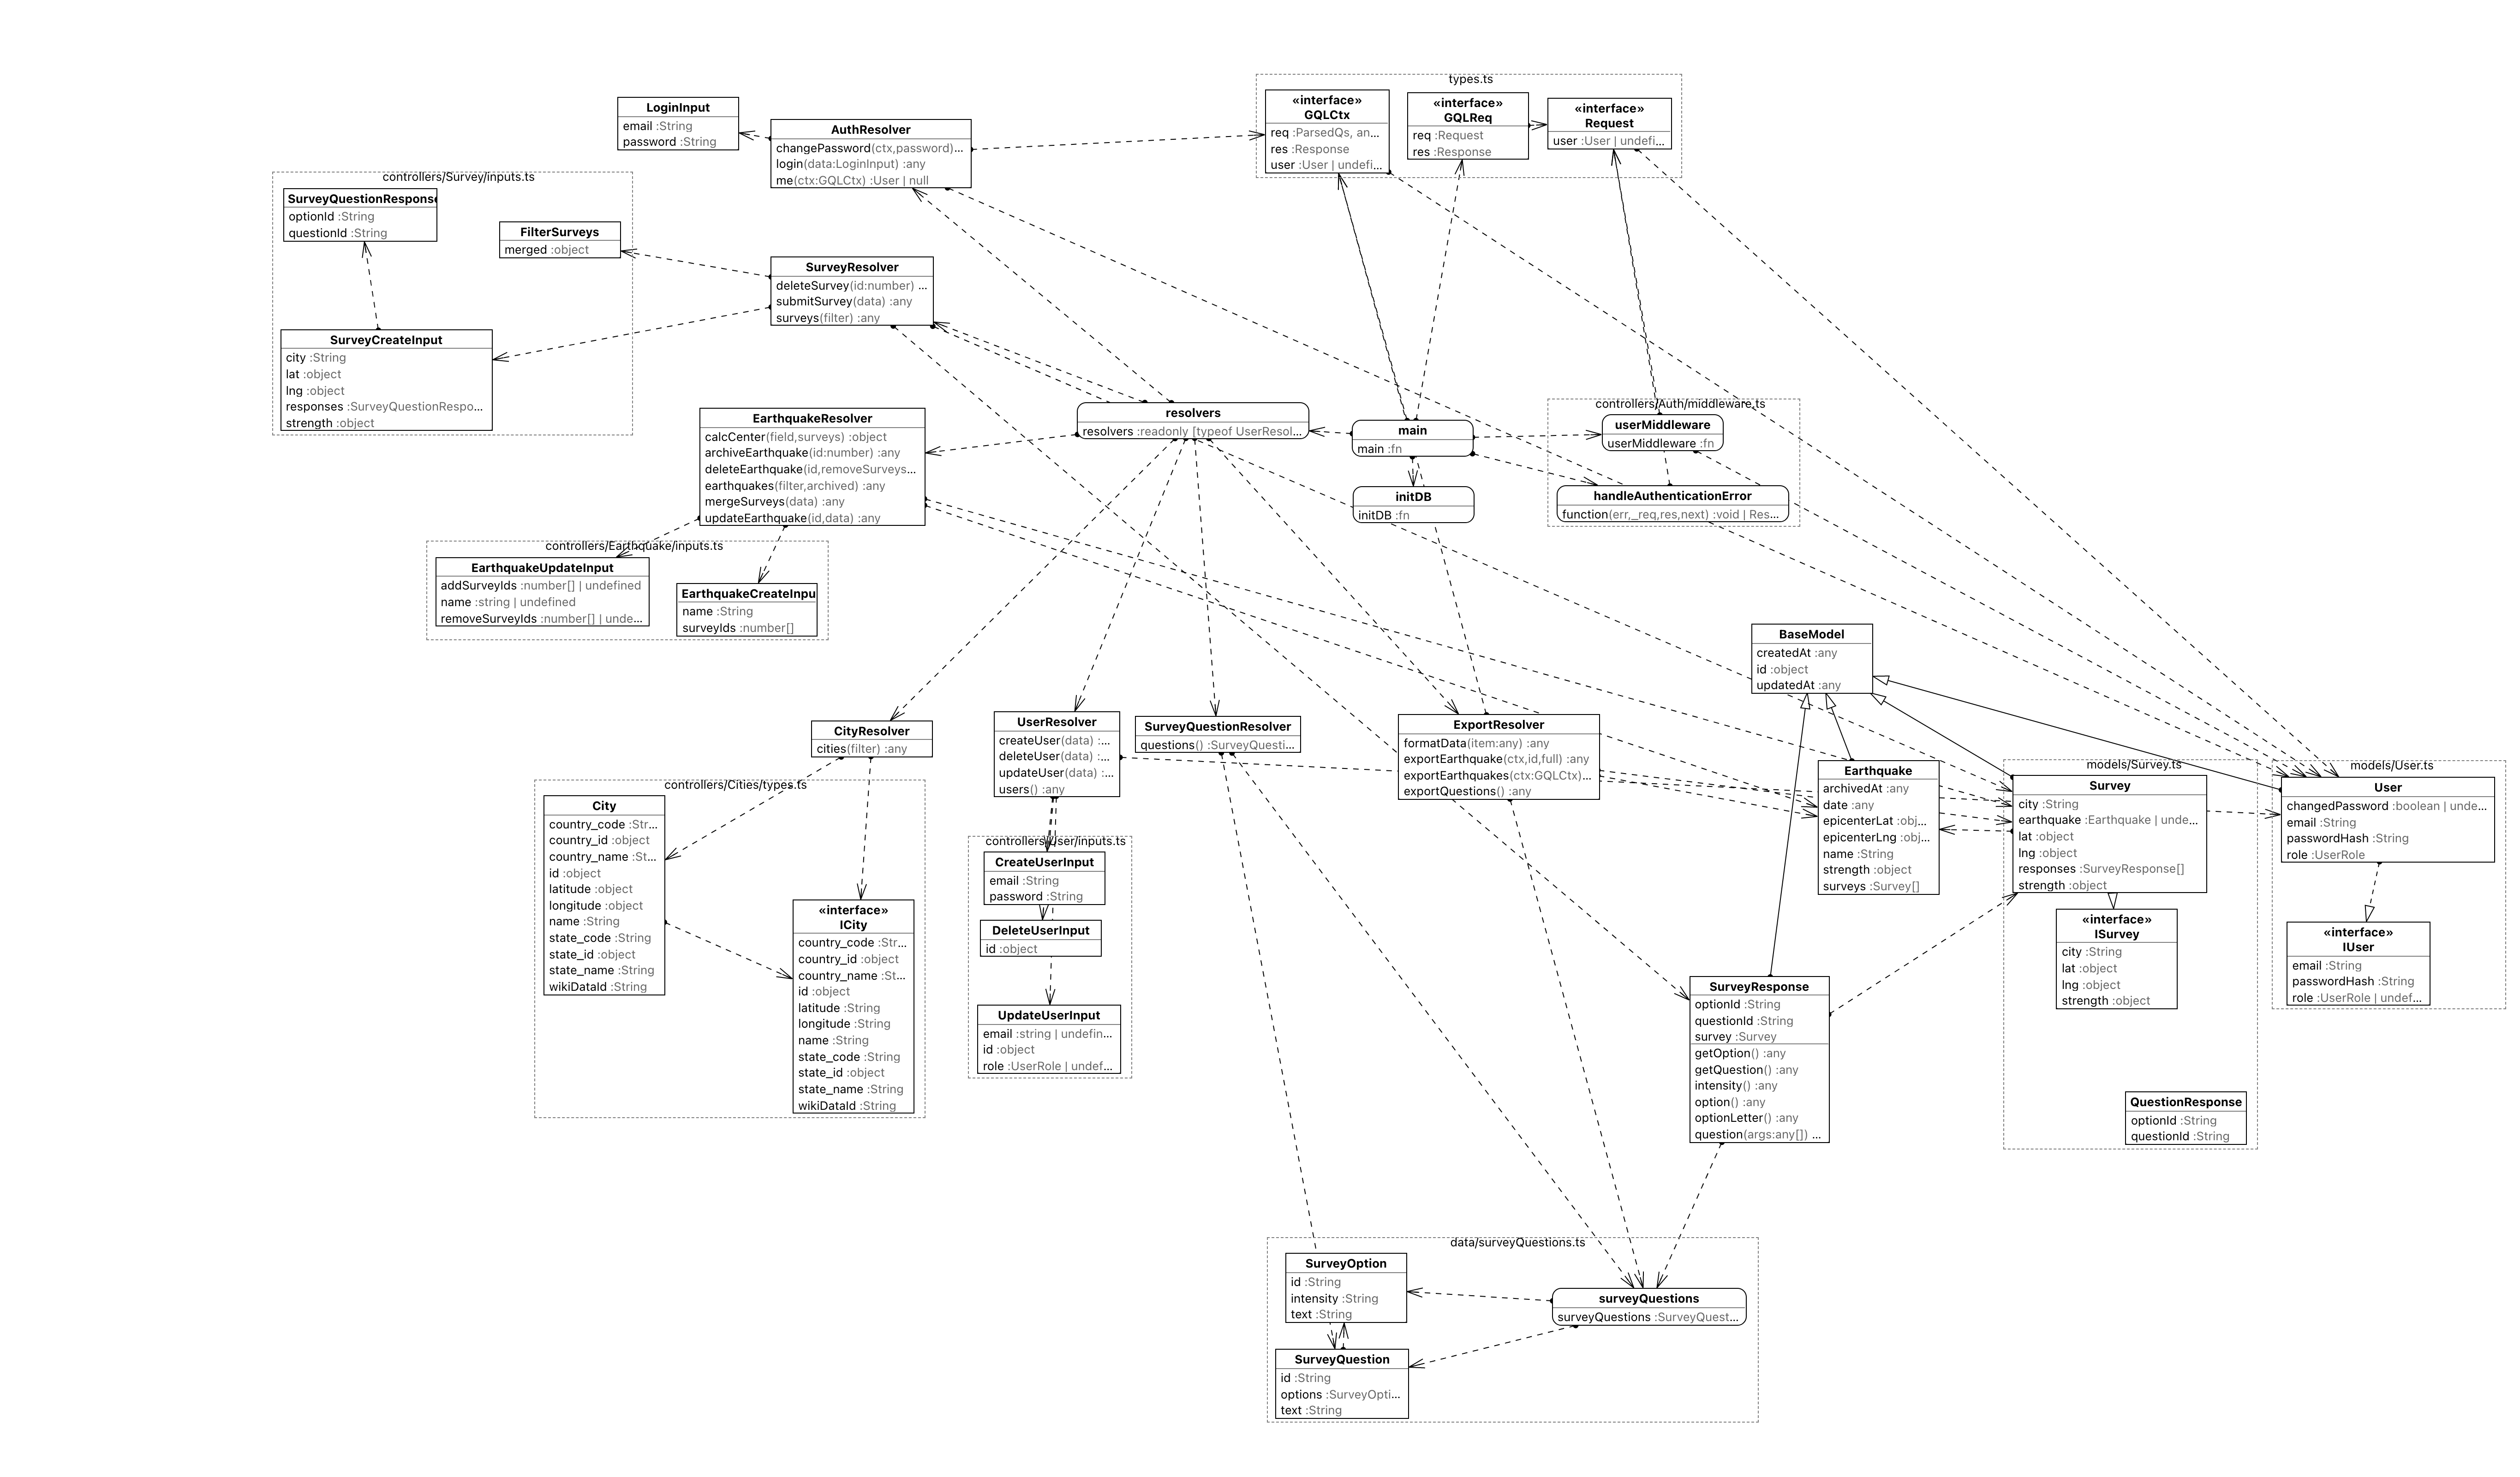
\includegraphics[width=\textwidth]{slike/classDiagram.png} 
				\caption{Dijagram razreda cijele aplikacije}
				\label{fig:uml} 
			\end{figure}

			\eject

		
		\section{Dijagram stanja}

		Dijagram stanja prikazuje stanja objekta te prijelaze iz jednog stanja u drugo temeljene na događajima. Na slici 4.6 prikazan je dijagram stanja za seizmologa koji je već prijavljen u sustav. Seizmolog je registrirani korisnik te ima više mogućnosti od građana koji nisu registrirani, ali manje od administratora. 
        
		Seizmologu se prvo, kao i ostalim korisnicima aplikacije, prikazuje Početna stranica. Na početnoj se stranici, kada joj netko pristupi, osvježe podatci na karti. Početna stranica seizmologu nudi pet opcija daljnjeg korištenja aplikacije te su one prikazane s pet stanja. 
        U gornjem desnom kutu može odabrati mogućnost promjene svoje lozinke. Pri kliku na tu opciju, odmah mu se otvara obrazac za promjenu lozinke.
        Ako u obrazac upiše ispravnu novu lozinku te pritisne "Spremi", podatci će se ažurirati i vratiti seizmologa na početnu stranicu. Ako u obrazac ne upiše ispravnu novu lozinku, ostaje na istoj stranica i njegova lozinka se ne mijenja
        
		Iz stanja Početna stranica, seizmolog klikom na "Novi potres?" prelazi u stanje Ispunjavanje novog upitnika. U tom se stanju korisniku prikazuje obrazac s pitanjima o potresu kojeg korisnik želi prijaviti. 
        Nakon što ispuni cijeli upitnih i pritisne "Spremi", aplikacija korisnika vraća u stanje Početna stranica.
        Ukoliko ipak odluči da ne želi ispuniti upitnik, utoliko će se povratkom na početnu stranicu ponovno naći u stanju Početna stranica. 
        
		Na početnoj stranici klikom na opciju "Arhivirani potresi", seizmolog prelazi u stanje Arhivirani potresi. U tom stanju odmah ulazi u podstanje Pregled arhiviranih potresa te mu se prikazuju svi arhivirani potresi te mogućnost pretraživanja tih potresa.
        Seizmolog ima mogućnost odabira i preuzimanja podataka o potresu (ispunjeni upitnici, lokacija, intezitet...). Preuzimanje podataka nalazi se u podstanju Odabran jedan arhivirani potres.
        
		Iduće stanje u kojem se seizmolog može naći je Aktualni potresi. U stanje Aktualni potresi prelazi odabirom opcije "Aktuali potresi". 
        Potom direktno prelazi u podstanje Pregled aktualnih potresa gdje mu se prikazuju aktualni potresi koje je, također, moguće filtirati kao i arhivirane. Kao i u stanju Arhivirani potresi, seizmologu se i u stanju Aktualni potresi nudi mogućnost 
        prelaska u podstanje Odabran jedan aktualni potres. U tom se podstanju provodi preuzimanje podataka o potresu. Iz stanja Aktualni potresi i Arhivirani potresi, seizmolog može prijeći u stanje Početna stranica.
       
		Osim u podstanjima Odabran jedan aktualni potres i Odabran jedan arhivirani potres, podaci se mogu preuzimati i u posebnom stanju Izvoz podataka. U to stanje seizmolog može doći klikom na "Izvoz podataka". 
        Podstanje u kojem će se seizmolog naći ovisi o tome je li "toggle" postavljen na "Preuzmi i upitnike" ili na "Izuzmi upitnike". U podstanju "Preuzmi i upitnike" prikazat će mu se stranica sa svim potresima te će klikom na "Preuzmi" preuzeti potrese zajedno sa pitanjima iz upitnika.
        Svi potresi se prikazuju i u podstanju "Preuzmi bez upitnika", no u tom će podstanju klikom na "Preuzmi" preuzeti samo podatke vezano uz potres, ali ne i pitanja. Iz oba podstanja klikom na "Preuzmi pitanja upitnika" prelazi se u podstanje "Preuzimanje pitanja upitnika".
        U tom podstanju preuzimaju se isključivo pitanja koja su u upitniku i svi mogući odgovori na njih. Iz tog postanja direktno se vraćamo na početak te, ovismo o ome je li "toggle" postavljen na "Preuzmi i upitnike" ili na "Izuzmi upitnike", odlazimo u jedno od tih podstanja.
        Iz stanja Izvoz podataka možemo prijeći u stanje Početna stranica.
        Završetak rada događa se klikom na "Odjavi se". Tu mogućnost seizmolog ima u svim stanjima.
			
			
			
		\begin{figure}[H]
            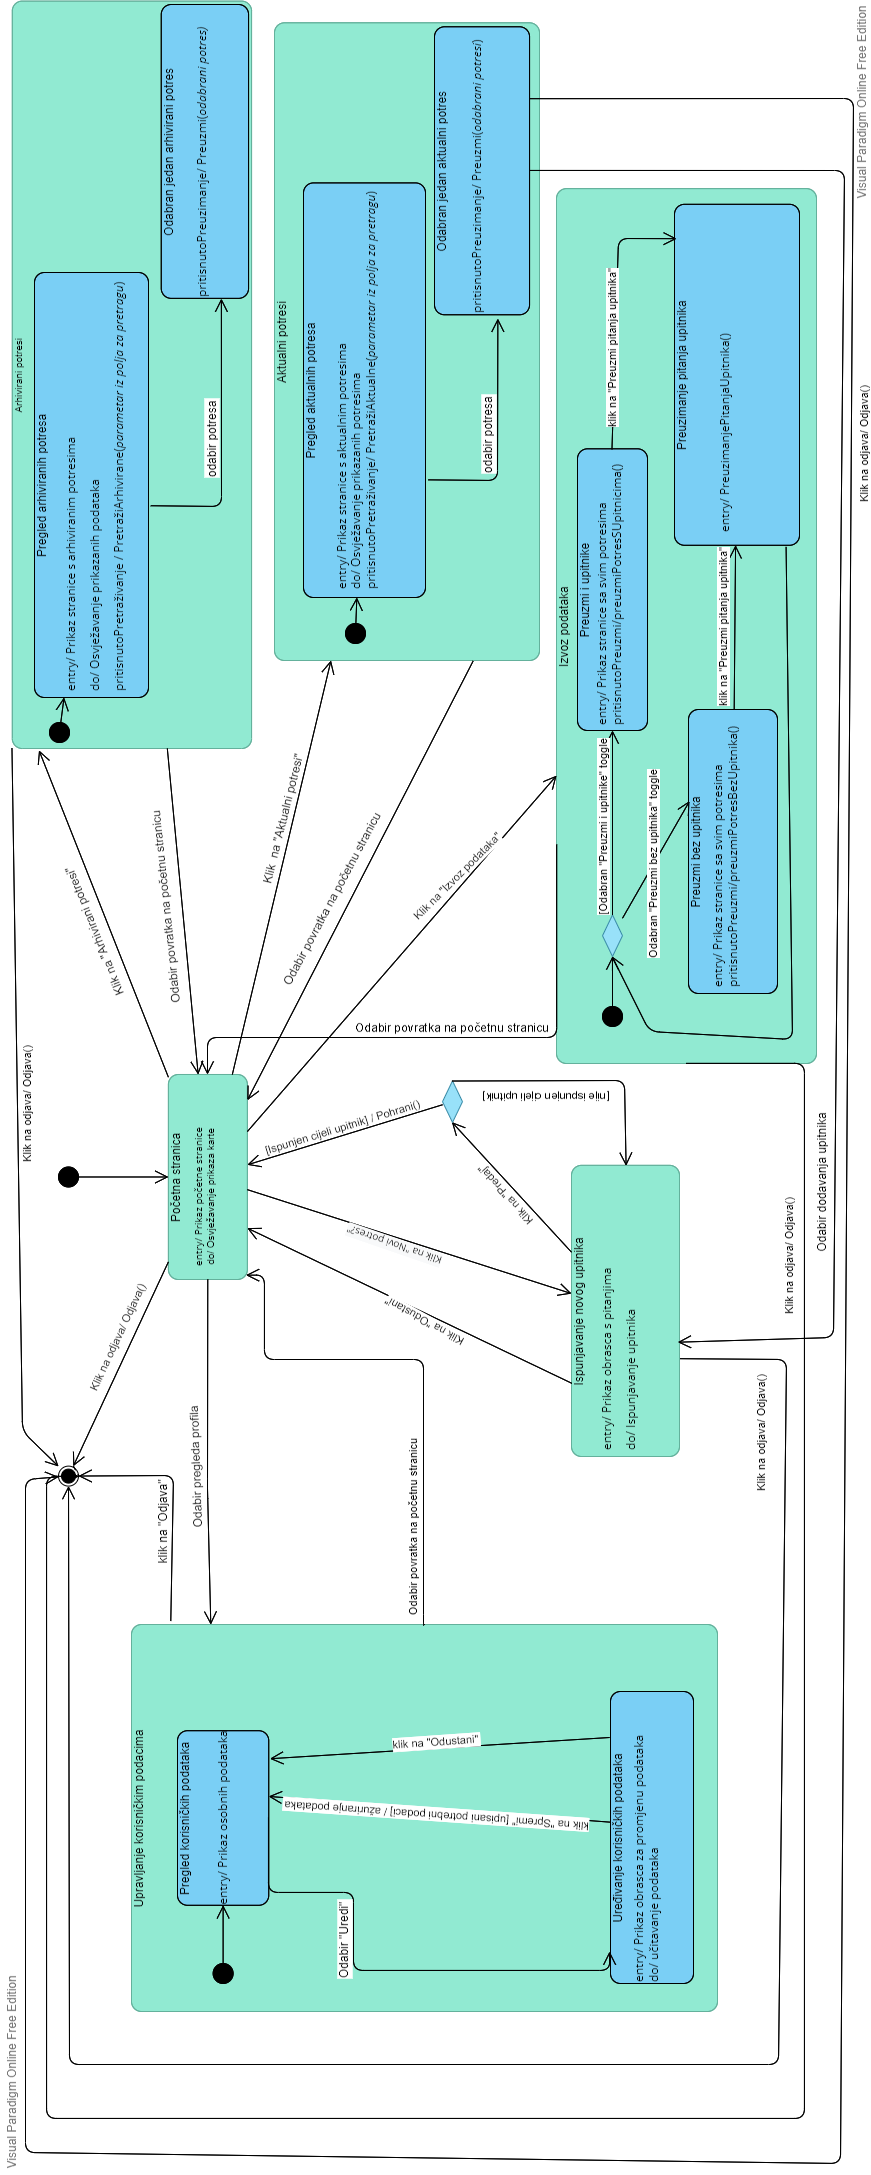
\includegraphics[width=\textwidth, height=15cm]{slike/dijagramstanja.png}
            \caption{Dijagram stanja}
            \label{fig:uml_db} 
        \end{figure}
			
			\eject 
		
		\section{Dijagram aktivnosti}
		
		Dijagram aktivnosti služi za modeliranje procesa. On opisuje ponašanje različitih elemenata modela toka upravljanja ili toka podataka. Ne upotrebljava se za modeliranje ponašanja poticanog događajima. Prilikom modeliranja toka upravljanja svaki novi korak poduzima se nakon završenog
		prethodnog. Na slici 4.7 prikazan je dijagram aktivnosti procesa pregleda aktualnih potresa, njihovog pretraživanja i preuzimanja podataka za njih. 
		Na ovom dijagramu "Korisnik" može biti i seizmolog i administrator.
		
		Prvo se korisnik prijavljuje u sustav. Nakon uspješne prijave, na početnoj stranici odabire "Aktualni potresi". Korisnik vidi prikaz stranice aktualnih potresa. Korisnik može pretraživati potrese prema nekom parametru. Ako nema potresa koji zadovoljavaju korisnikov upit, sustav javlja korisniku da takvih potresa nema. Potresi s traženim svojstvima prikazat će se ako postoje potresi koji zadovoljavaju upit (npr. pretraga po nazivu, mjestu, jačini...). Ako korisnik ne želi filtrirati potrese, jednostavno neće upisati nikakav upit u tražilicu te će se i dalje prikazivati lista svih aktualnih potresa.
		
		Kada je pronašao željeni potres te ga označio, klikom na "Preuzmi" korisnik pokreće preuzimanje podataka za odabrani potres. Podatci se preuzimaju u .csv formatu. Korisnika se obavještava o uspješnom preuzimanju podataka.
		
		\begin{figure}[H]
			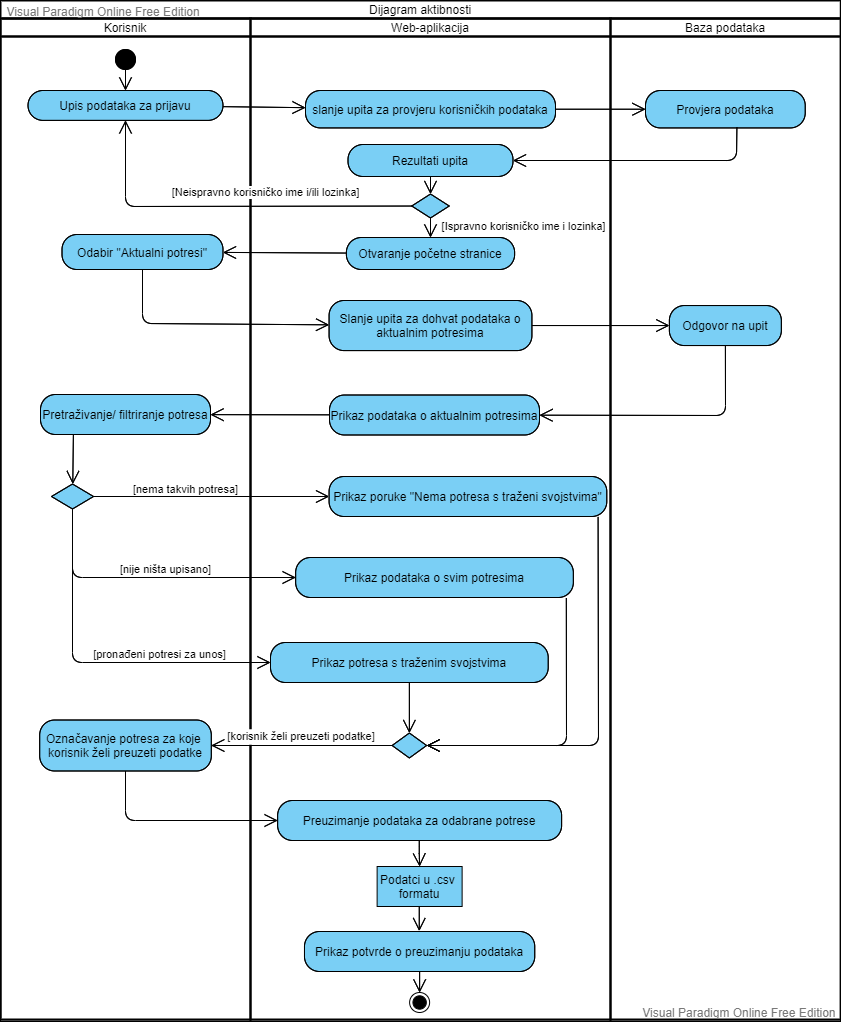
\includegraphics[width=\textwidth]{slike/dijagram_aktivnosti.png}
			\caption{Dijagram aktivnosti}
			\label{fig:uml_db} 
		\end{figure}
		
			
			\eject
		\section{Dijagram komponenti}
		
			\textbf{\textit{dio 2. revizije}}\\
		
			 \textit{Potrebno je priložiti dijagram komponenti s pripadajućim opisom. Dijagram komponenti treba prikazivati strukturu cijele aplikacije.}
		\eject